\section{Static control flow analysis}

Consider the program Control Flow Graph (CFG) below, with seven nodes:
\begin{figure}[H]
    \centering
    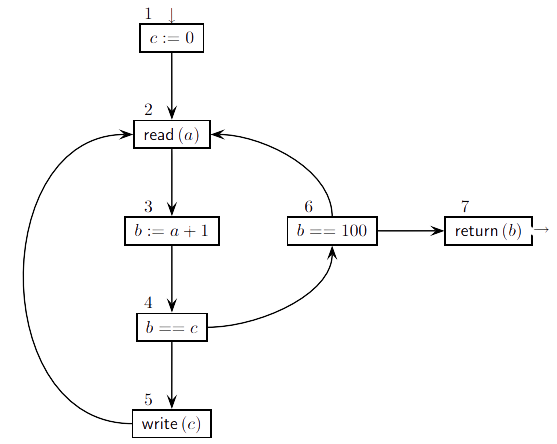
\includegraphics[width=0.65\linewidth]{images/CFG.png}
\end{figure} 
Answer the following questions:
\begin{enumerate}
    \item Informally find the live variables at the input of each node of the CFG.
    \item Can variables a and b share the same memory cell?
    \item Find again the live variables at the input of each CFG node, through the data-flow equation method. Verify that the result is coherent with point one. 
\end{enumerate}

\paragraph*{Solution}
\begin{enumerate}
    \item At the input of node 1 (initial) no variable is live, since every variable is assigned in the initial node itself or in some successor thereof before using.
        At the output of node 7 (final), by definition no variable is live. The other liveness intervals are just an application of the liveness definition. 
        For instance, variable c is live at the inputs of all the nodes in the two loops (2-3-4-5 and 2-3-4-6), since it is used inside both loops (in the node 4) 
        and is never reassigned after being initialized in the node 1 outside the loops. Variables a and b are even simpler: $a$ is assigned in 2 and is used in 3,
        thus it is live only at 3; and $b$ is assigned in 3 and is used in 4, 6 and 7, respectively first, second and third successor of 3, thus it is live at 4, 6 
        and 7 themselves.
        \begin{figure}[H]
            \centering
            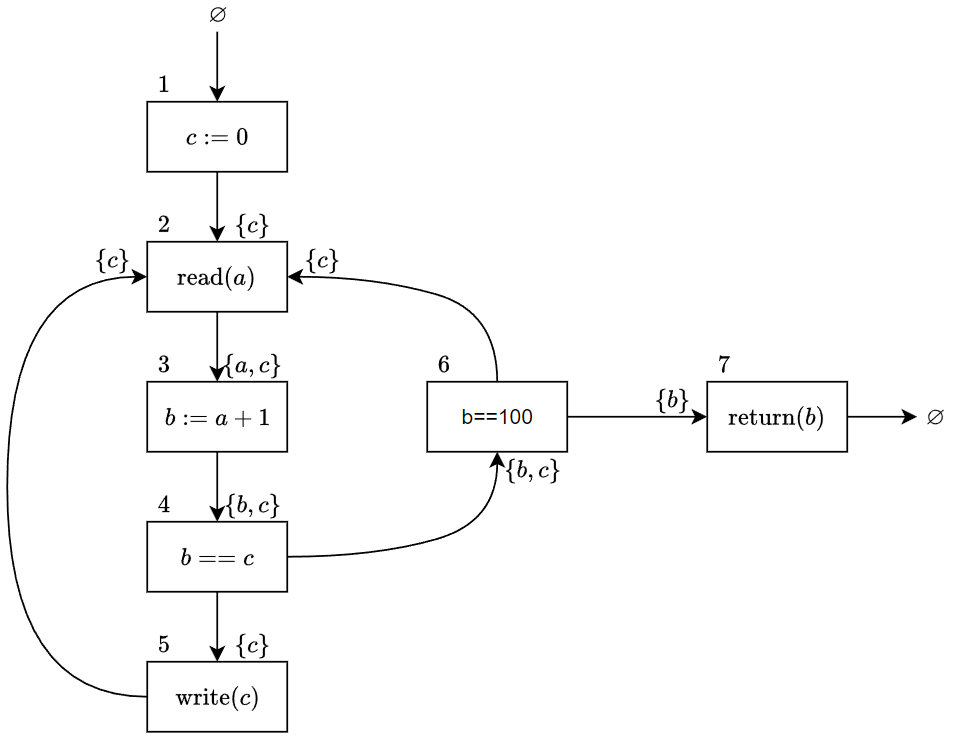
\includegraphics[width=0.75\linewidth]{images/CFGlive.png}
        \end{figure} 
    \item Yes, variables $a$ and $b$ can share the same location. In fact, they are not simultaneously live at any program node, thus they can share the same 
        memory cell or processor register.
    \item We can construct the following table: 
        \begin{table}[H]
            \centering
            \begin{tabular}{l|c|c|}
            \cline{2-3}
                                    & \textbf{Defined} & \textbf{Used} \\ \hline
            \multicolumn{1}{|l|}{1} & $c$              &               \\
            \multicolumn{1}{|l|}{2} & $a$              &               \\
            \multicolumn{1}{|l|}{3} & $b$              & $a$           \\
            \multicolumn{1}{|l|}{4} &                  & $b,c$         \\
            \multicolumn{1}{|l|}{5} &                  & $c$           \\
            \multicolumn{1}{|l|}{6} &                  & $b$           \\
            \multicolumn{1}{|l|}{7} &                  & $b$           \\ \hline
            \end{tabular}
        \end{table}
        We have that: 
        \begin{table}[H]
            \centering
            \begin{tabular}{|c|l|l|}
            \hline
            \textbf{Node} & \multicolumn{1}{c|}{\textbf{In equations}}                 & \multicolumn{1}{c|}{\textbf{Out equations}}                \\
            $i$           & $\text{in}(i)=(\text{out}(i)-\text{def}) \cup \text{used}$ & $\text{out}(i)=\bigcup_{j \in \text{succ}(i)}\text{in}(j)$ \\ \hline
            1             & $\text{in}(1)=\text{out}(1)-\{c\}$                         & $\text{out}(1)=\text{in}(2)$                               \\
            2             & $\text{in}(2)=\text{out}(2)-\{a\}$                         & $\text{out}(2)=\text{in}(3)$                               \\
            3             & $\text{in}(3)=(\text{out}(3)-\{b\})\cup\{a\}$              & $\text{out}(3)=\text{in}(4)$                               \\
            4             & $\text{in}(4)=\text{out}(4)\cup\{b,c\}$                    & $\text{out}(4)=\text{in}(5)\cup\text{in}(6)$               \\
            5             & $\text{in}(5)=\text{out}(5)\cup\{c\}$                      & $\text{out}(5)=\text{in}(2)$                               \\
            6             & $\text{in}(6)=\text{out}(6)\cup\{b\}$                      & $\text{out}(6)=\text{in}(7)\cup\text{in}(2)$               \\
            7             & $\text{in}(7)=\text{out}(7)\cup\{b\}$                      & $\text{out}(7)=\varnothing$                                \\ \hline
            \end{tabular}
        \end{table}
        And the iterations are: 
        \begin{table}[H]
            \centering
            \begin{tabular}{ccccccccccc}
            \textbf{}                 & \multicolumn{2}{c}{\textbf{Initialization}} & \multicolumn{2}{c}{\textbf{1}}   & \multicolumn{2}{c}{\textbf{2}}   & \multicolumn{2}{c}{\textbf{3}}   & \multicolumn{2}{c}{\textbf{4}} \\
            \multicolumn{1}{c|}{$\#$} & out       & \multicolumn{1}{c|}{in}         & out  & \multicolumn{1}{c|}{in}   & out  & \multicolumn{1}{c|}{in}   & out  & \multicolumn{1}{c|}{in}   & out             & in           \\ \hline
            \multicolumn{1}{c|}{1}    & -         & \multicolumn{1}{c|}{-}          & -    & \multicolumn{1}{c|}{-}    & -    & \multicolumn{1}{c|}{-}    & $c$  & \multicolumn{1}{c|}{-}    & $c$             & -            \\
            \multicolumn{1}{c|}{2}    & -         & \multicolumn{1}{c|}{-}          & $a$  & \multicolumn{1}{c|}{-}    & $ac$ & \multicolumn{1}{c|}{$c$}  & $ac$ & \multicolumn{1}{c|}{$c$}  & $ac$            & -            \\
            \multicolumn{1}{c|}{3}    & -         & \multicolumn{1}{c|}{$a$}        & $bc$ & \multicolumn{1}{c|}{$ac$} & $bc$ & \multicolumn{1}{c|}{$ac$} & $bc$ & \multicolumn{1}{c|}{$ac$} & $bc$            & -            \\
            \multicolumn{1}{c|}{4}    & -         & \multicolumn{1}{c|}{$bc$}       & $bc$ & \multicolumn{1}{c|}{$bc$} & $bc$ & \multicolumn{1}{c|}{$bc$} & $bc$ & \multicolumn{1}{c|}{$bc$} & $bc$            & -            \\
            \multicolumn{1}{c|}{5}    & -         & \multicolumn{1}{c|}{$ c$}       & -    & \multicolumn{1}{c|}{$ c$} & -    & \multicolumn{1}{c|}{$ c$} & $ c$ & \multicolumn{1}{c|}{$ c$} & $ c$            & -            \\
            \multicolumn{1}{c|}{6}    & -         & \multicolumn{1}{c|}{$b$}        & $b$  & \multicolumn{1}{c|}{$b$}  & $b$  & \multicolumn{1}{c|}{$b$}  & $bc$ & \multicolumn{1}{c|}{$bc$} & $bc$            & -            \\
            \multicolumn{1}{c|}{7}    & -         & \multicolumn{1}{c|}{$b$}        & -    & \multicolumn{1}{c|}{$b$}  & -    & \multicolumn{1}{c|}{$b$}  & -    & \multicolumn{1}{c|}{$b$}  & -               & -           
            \end{tabular}
        \end{table}
        The out columns at steps 3 and 4 coincide, thus the iteration process converges in three steps. The in column at step 3 lists all the variables
        live at the program node inputs. The live variable latest to reach a node input is $c$ at node 6 (compare the in columns at steps 2 and 3). In fact, 
        variable $c$ propagates backwards from node 4, where it is used, to node 6, and to do so it has to cross nodes 3 and 2 in succession, which just takes 
        three steps in total. All the other propagation cases are fast. The systematic solution obtained through the data-flow method is identical to the informal 
        one of point one. 
\end{enumerate}